\section{Component Architecture} \label{ComponentArchitecture}
In this section a class diagram will be designed to show the specifications of all complex components. This is done in order to create a flexible and understandable structure of the system.

\begin{figure}[H]
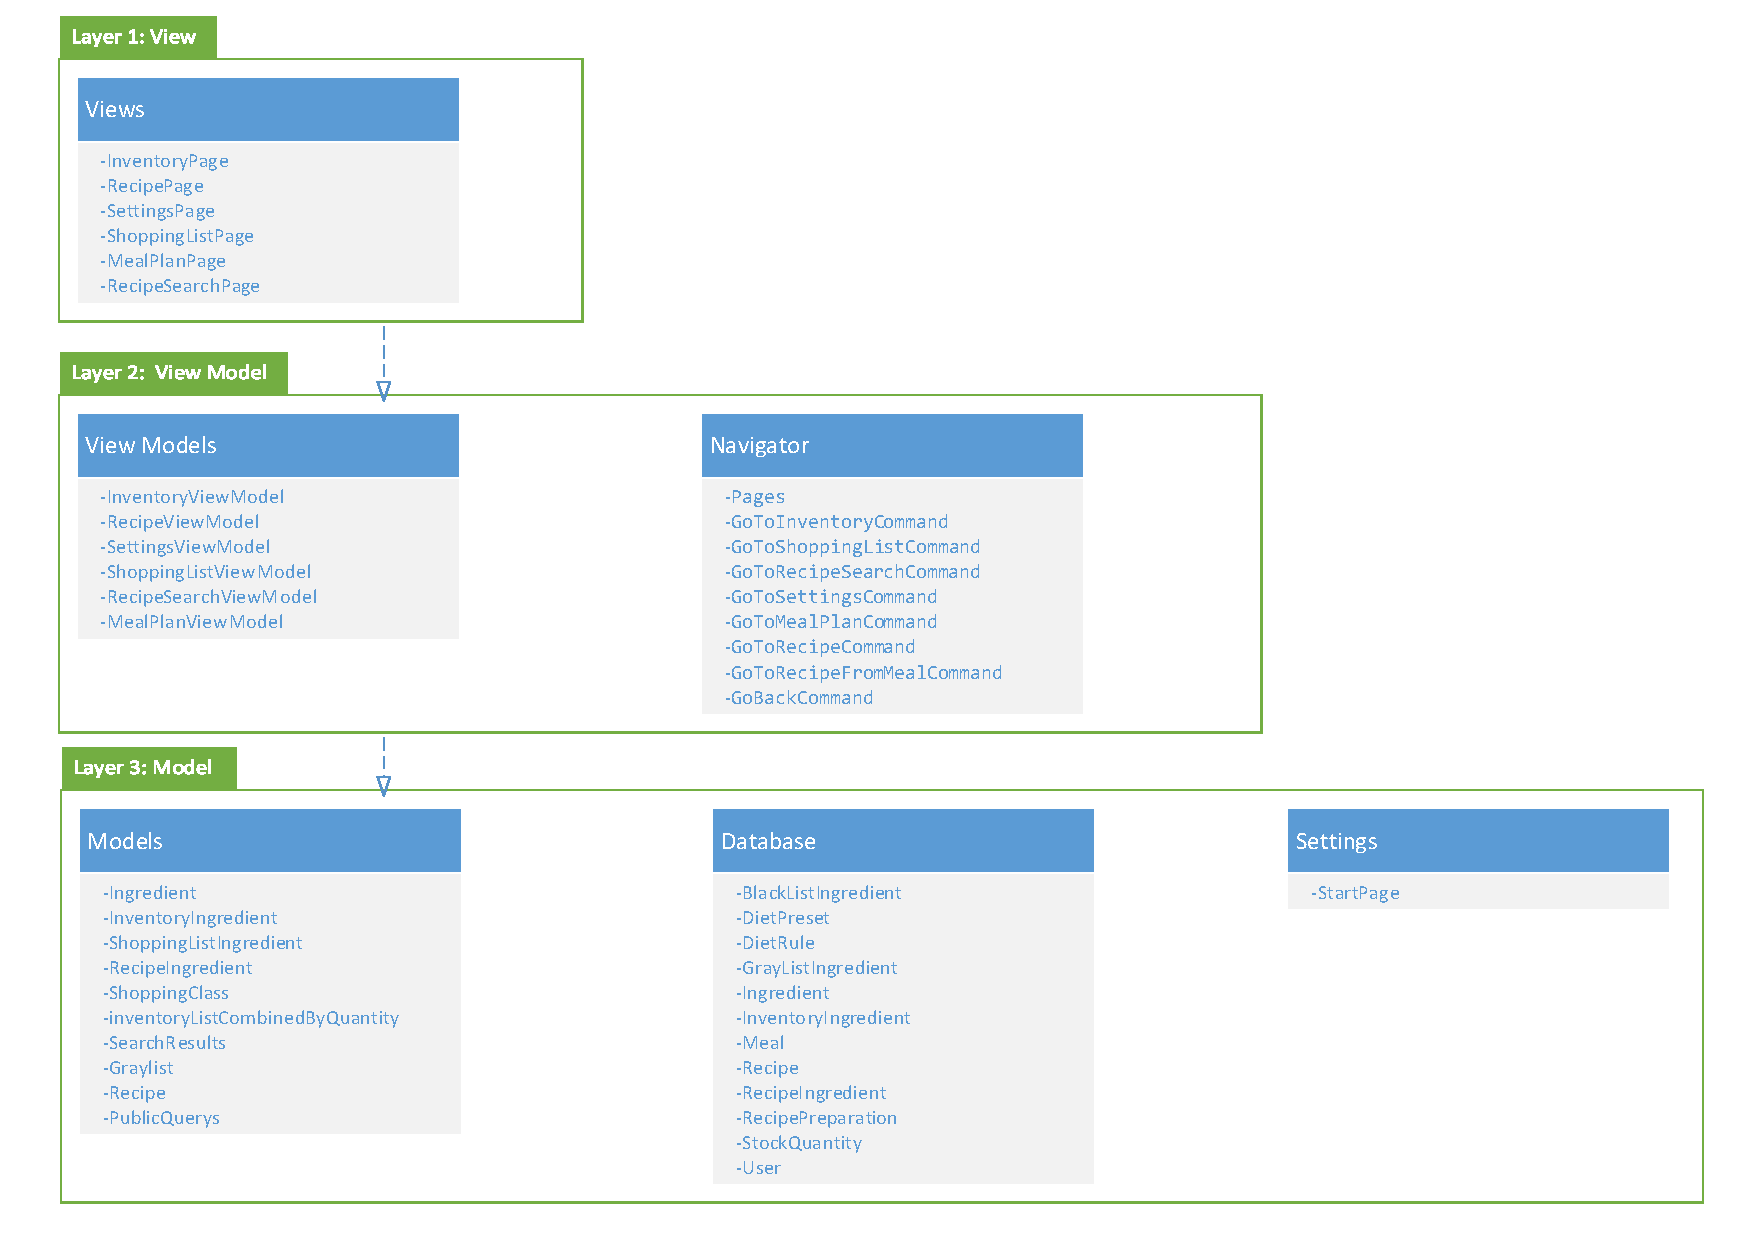
\includegraphics[width=\linewidth]{Grafik/FoodPlanner/ComponentDiagram}
\centering
\caption{Class layer diagram}
\label{LayerDiagram}
\end{figure}

\Cref{LayerDiagram} shows the class diagram for the components of the system. The pattern used is the MVVM pattern which is described in \cref{MVVMSection}.

\textbf{View:}
The View component spans over the pages that are used to interact with the user. The View is responsible for sending information to the ViewModel such that the user can interact with the system. It also displays data from properties in the ViewModel using databinding.

\textbf{ViewModel:}
The ViewModel component spans over the classes that are associated with the pages in the view. The responsibility of the ViewModel is to read and update data in the model. The component uses the classes found in the Model. The ViewModel also contains a Navigator which is used by the View and ViewModel itself and is responsible for letting the user navigate trough the different pages.

\textbf{Model:}
All the classes in the system described in \cref{ClassesLabel} are going to be located in the Model component and is used directly by the ViewModel. The responsibility of the Model is to provide classes that can be used to manipulate data and synchronise such data with a database. The objects that can be created through the Model are used in the ViewModel. Another part of the Model is the settings. The settings are saved locally on the machine and are responsible for allowing some personal customization of the local processor.

There is an external standard component which is not shown on the diagram, the component is the Entity Framework which will be used to simplify the data handling when data is saved or retrieved from/to the database, \cref{EntityFrameworkSection} describes the framework in more detail.